\section{Sponsor}

The CGU Math Clinic project is sponsored by Sandia National Laboratories (SNL) in Albuquerque, New Mexico. SNL is managed and operated by the National Technology and Engineering Solutions of Sandia, an owned subsidiary of Honeywell International, Inc. Sandia was originally founded in 1949, and their current effort is to develop, engineer, and test non-nuclear components of nuclear weapons. Sandia responds to federal government solicitations, and one of their most recent projects is studying fractures in silica-based glasses. To optimize computation efficiency, Sandia aims to utilize machine learning (ML) algorithms which will lend to a greater understanding as to why and how fractures nucleate and propagate.

%%%Example from 20117-18 report%%%
%to further the US nuclear program, LANL's interest in modeling brittle damage centers around ensuring weapons safety and adherence to global nuclear testing standards by examining static fracture networks, modeling dynamic fracture propagation, and understanding uncertainty quantification and data assimilation. LANL currently has accurate, yet computationally intense methods of doing so. In the 2017-2018 project year, our focus is on modeling dynamic fracture propagation using Machine Learning (ML) methods based on LANL modeling data, to  reduce computational load dramatically while retaining that accuracy.

\section{Background}
Silicate glasses are used widely, in fields that include medicine, optics, electronics, telecommunication and energy. While these materials have numerous benefits in terms of strength and resilience, they are also brittle. When placed under sufficient tensile stress, glasses fracture rather than stretch. The fractures grow, propagating through the glass and ultimately leading to material failure. In spite of considerable study, the nanoscale origins of fracture and the relation of atomic structure to fracture nucleation remain poorly understood.

A natural hypothesis might be that fracture nucleation is related to the presence of atomic-scale defects or chemical bond weakness in the glass. However, the relationship between atomic structure and fracture behavior is complex. Fractures do not simply originate at the site of the weakest link or most easily broken bond, and trigger further fracturing in the surrounding bonds~\cite{markpres}. Similarly, glasses with an increased density of nanoscale voids and defects do not necessarily display increased brittle behavior, and can even be better at absorbing stresses from mechanical deformation~\cite{pedone2015dynamics}. Instead, the nucleation and propagation of fractures appear to depend on more subtle characteristics of the local structure surrounding an atom.

\subsection{Physical Structure}
The basic molecular unit in a silicate glass is a silicon (Si) atom bonded to four oxygen (O) atoms in a tetrahedral configuration.  Each of these SiO$_4$ units can share its O atoms with neighboring tetrahedra.  An O atom shared between two molecules in this way is known as a \emph{bridging oxygen}, as seen in Figure~\ref{fig:tetrahedra}.

\begin{figure}[!b]
    \centering
    \noindent
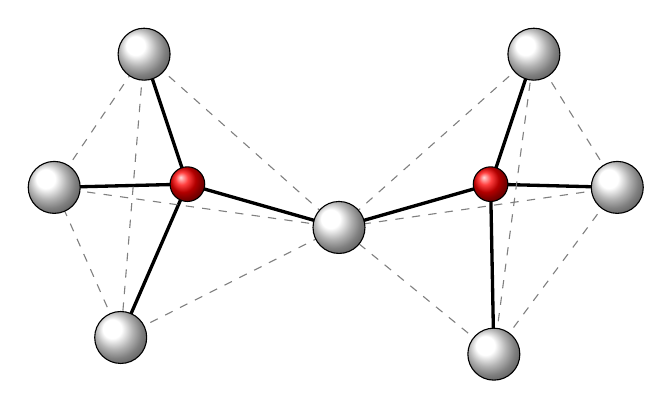
\begin{tikzpicture}[scale=1.1]
\coordinate (A) at (-0.5,0.5,0); % Left back O 
\coordinate (B) at (2,0.5,4.5); % Left front O  
\coordinate (C) at (6,0.5,0); % Right back O
\coordinate (D) at (6.5,0.5,5); % Right front O 
\coordinate (E) at (3.75,1,2.5); % Bridging Oxygen 
\coordinate (F) at (5.5,1.5,2.5); % Right Si
\coordinate (G) at (2,1.5,2.5); % Left Si 
\coordinate (H) at (1.5,3,2.5); % Left top O 
\coordinate (I) at (6,3,2.5); % Right Top O

%connections from left Si
\draw [very thick] (G) -- (A);
\draw [very thick] (G) -- (B);
\draw [very thick] (G) -- (H);
\draw [very thick] (G) -- (E);

%connections from Right Si 
\draw [very thick] (F) -- (C);
\draw [very thick] (F) -- (D);
\draw [very thick] (F) -- (I);
\draw [very thick] (F) -- (E);

%dashed lines between Oxygen. This can be removed but it was in literature. 
\draw[gray,dashed] (A) -- (H);
\draw[gray,dashed] (H) -- (B);
\draw[gray,dashed] (B) -- (A);
\draw[gray,dashed] (A) -- (E);
\draw[gray,dashed] (H) -- (E);
\draw[gray,dashed] (B) -- (E);

\draw[gray,dashed] (I) -- (C);
\draw[gray,dashed] (C) -- (D);
\draw[gray,dashed] (D) -- (I);
\draw[gray,dashed] (I) -- (E);
\draw[gray,dashed] (D) -- (E);                                                
\draw[gray,dashed] (C) -- (E);                                                

%place non-atom cube corners
\shadedraw [ball color= white] (A) circle (0.3cm);
\shadedraw [ball color= white] (B) circle (0.3cm);
\shadedraw [ball color= white] (C) circle (0.3cm);
\shadedraw [ball color= white] (D) circle (0.3cm);
\shadedraw [ball color= white] (E) circle (0.3cm);
\shadedraw [ball color= red] (F) circle (0.20cm);
\shadedraw [ball color= red] (G) circle (0.20cm);
\shadedraw [ball color= white] (H) circle (0.3cm);
\shadedraw [ball color= white] (I) circle (0.3cm);
\end{tikzpicture}
    \caption{Two silicon atoms (small red balls) with surrounding oxygen atoms (large grey balls) in tetrahedral configuration.  One bridging oxygen is at a corner shared by the two tetrahedra.}
    \label{fig:tetrahedra}
\end{figure}

When an Si atom is surrounded by $n$ bridging O atoms, it is called a Q$_n$ unit~\cite{shelby2005}. In a network of Q$_4$ units, all O atoms are shared between two Si atoms, forming a silicon dioxide (SiO$_2$) structure.  The network geometry can be regular, in which case the material is a crystal such as quartz.  Alternatively, the geometry can be irregular, in which case it is a glass.  When the network has Q$_n$ units with $n<4$, some of the O atoms surrounding an Si atom are non-bridging.

An Si atom can also be undercoordinated, bonding with fewer than four O atoms, or overcoordinated, breaking the tetrahedral symmetry and bonding with more than four O atoms.  In the latter case, this can result in rare Q$_n$ units with $n>4$~\cite{pedone2015dynamics}.

\subsection{Molecular Dynamics Simulations} 

The conventional approach for studying the fracture mechanics of materials has been to model their structure as a continuum, ignoring atomic detail, and predicting strength and failure using a theoretical description at the macroscopic scale.  For high-fidelity predictions of fracture dynamics in silica-based glasses, however, continuum theory encounters limitations~\cite{shimada2015breakdown}.

Molecular dynamics (MD) methods instead provide an atomistic approach, simulating the system at the nanoscale and modeling the individual chemical and physical interactions taking place in the material. These simulations have successfully predicted a wide range of detailed properties that cannot be obtained with continuum methods, and that are consistent with experimental observations~\cite{pedone2009properties}.

In order to model a silicate glass, MD simulates heating quartz to a very high temperature, far above its melting point.  The melt is then rapidly cooled, or \emph{quenched}, to room temperature, introducing the molecular disorder that characterizes glassy structure.  While the quench rate that can feasibly be simulated (3.7~K/picosecond) is orders of magnitude faster than experimental reality, it nevertheless provides results that are in many cases a good match with experimental data~\cite{markpres,mWilson_continuum_stress}

%%  CRACK PROPAGATION SIMULATION FIGURE 

\begin{figure}
    \centering
    \noindent
\includegraphics[width=0.45\textwidth]{frac_prop1.PNG}\hspace{0.15\textwidth}%
\includegraphics[width=0.4\textwidth]{frac_prop2.PNG}\\[2em]
\includegraphics[width=0.4\textwidth]{frac_prop3.PNG}\hspace{0.2\textwidth}%
\includegraphics[width=0.4\textwidth]{frac_prop4.PNG}\par
    \caption{Four snapshots showing the progression of an MD simulation of fracture propagation, in a 3D silicate glass sample. The material is loaded in uniaxial tension in the horizontal direction, with free surfaces in the two other directions.}
    \label{fig:crack_prop}
\end{figure}

Once the silicate glass is generated in this way, its dynamics may be simulated under a range of environmental conditions.  Figure~\ref{fig:crack_prop} shows several snapshots from an MD simulation representing a three-dimensional system of size approximately 15 $\times$ 15 $\times$ 4~nm$^3$, containing approximately 70,000 atoms, under uniaxial tension in the horizontal direction.  As the material is deformed, a fracture nucleates starting from the lower boundary.  The void then propagates upwards, while another void nucleates in the bulk.  Although these two voids do not coalesce during the 1~nanosecond time interval represented by the simulation, they would likely do so subsequently, leading to failure in the material.

An environmental condition of particular interest in simulating glass fracture dynamics is the presence of water, and its effects on fracture growth. Water weakens the bonds between silicon and oxygen, lowering the energy barrier for bond breakage. MD simulations have shown that silicates in contact with an aqueous environment are more susceptible to fracture, both at the boundary and within the bulk~\cite{chem_effects}. This suggests that chemical effects can complicate the mechanical stress effects in modeling fracture dynamics. Simulations of the chemical-mechanical effects on crack tips have shown differing rates of fracture propagation, as well as changes in fracture direction and stress distribution in the atoms in the process zone where fractures propagate. Other effects of water are corrosive and can take up to microseconds to be measurable~\cite{markpres}, far beyond the time scale of simulations such as the one shown in Figure~\ref{fig:crack_prop}.

\subsection{Machine Learning Methods} 

MD simulations require vast amounts of computation. For example, running the simulation shown in Figure~\ref{fig:crack_prop} takes approximately 10,000 CPU hours. Moreover, each MD simulation represents only one particular configuration of atoms, given a set of material properties such as Young's modulus and density. In order to obtain statistically reliable estimates of macroscopic material behavior, it would be necessary to simulate thousands if not millions of configurations consistent with these properties.  Clearly, this would render MD computationally prohibitive.

An attractive alternative is to use machine learning (ML) as a surrogate model.  In this approach, a supervised learning algorithm is trained using data from a moderately-sized set of MD simulation results.  Once trained, the algorithm can rapidly predict certain outcomes of the simulation simply from the initial state of the system.  Surrogate models have been used extensively in applications ranging from aircraft design~\cite{mack2007surrogate} to hydrology~\cite{razavi2012review}.  These models can be as simple as polynomial functions to which data points are fitted by regression, or can be complex statistical models with thousands of tunable parameters.  What they have in common is that they do not attempt to model an underlying physical mechanism but rather to reproduce, in an approximate sense, the results of the simulations that they imitate.

Recent years have seen a number of successful research efforts using ML, often coupled with graph theoretic approaches, to predict fracture properties in materials. Wang et al.~\cite{MLACrack} have studied the use of ML methods for predicting fatigue crack growth rates. Work originating in a 2016-17 CGU Math Clinic project~\cite{valera2018machine,TopSystem} has used supervised learning methods to provide rapid predictions of high-flow regions of a fracture network representing subsurface rock, based on graph centrality features and limited training data from high-fidelity simulations.  Ebrahem et al.~\cite{ebrahem2018influence} and Bauchy~\cite{bauchy} have demonstrated the role of topological features in glass networks, in order to understand how local atomic structure affects deformation and resistance to fracturing.  The use of ML in the design of new glasses has been the subject of further study~\cite{liu2019machine}.  Finally, in a 2017-18 CGU Math Clinic project, Schwarzer et al.~\cite{schwarzer2019learning,mudunuru2019} used a graph theoretic description of brittle materials, training a deep neural network to recognize the dynamics of fracture propagation based on data from discrete finite-element simulations.  These results suggest that ML methods can productively complement MD simulations, providing accurate surrogate models that can be trained to mimic the behavior of MD while using dramatically less computation time.


\section{Goals}
The objective of our project is to develop supervised learning methods, trained on MD simulation data, that generate rapid predictions of where and when atomic-scale fractures occur in samples of silicate glasses under stress.  We aim to generate these predictions under multiple environmental conditions, and to validate them on existing MD simulation results.  Ultimately, we hope to relate our predictions to specific features characterizing local atomic structure, thus providing new insight into how this local structure leads to fracture and failure.

We separate our overall objective into the following two goals:

\begin{itemize}
\item \textbf{Goal 1:} \emph{Predict fracture nucleation events.} 

A nucleation event is where a new fracture, or void, emerges in the simulated system.  We aim to predict whether, based on the initial state of the system, a given atom lies on the boundary of a fracture at a certain later time in the simulation.  In order to do this, we assume that a nucleation event is primarily influenced by local atomic structure.  The definition of local could involve up to the $k$th neighbor of an atom, for some value of $k$.  The goal is to use network feature information of this kind to train a classifier to predict whether or not an atom ultimately forms part of a nucleation event.  We will also consider the closely related regression problem of estimating the probability that the atom forms part of a nucleation event.

\item \textbf{Goal 2:} \emph{Predict fracture propagation.} 

Fracture propagation is a continuing process of incorporating atoms into the fracture region, also known as the process zone.
Once a fracture nucleates at the surface or within the bulk of the material, it grows with the continued application of mechanical stress.  We aim to identify which new atoms will lie on the fracture's boundary, meaning the surface of a crack face, as it propagates.  Our goal is to train a supervised learning algorithm to learn the dynamics of fracture propagation from the full time series of feature values, so that it can then predict a time series from $t=0$ feature values alone.
\end{itemize}




